\documentclass[aspectratio=169]{beamer}
\usetheme{Madrid}
\usepackage{pgfplots}
\pgfplotsset{compat=1.18}
\usepackage{booktabs}
\usetikzlibrary{arrows.meta, positioning, calc, decorations.pathreplacing}

\title{Stepped scan vs.\ time-domain (FFT) scan}
\subtitle{How a modern EMI receiver measures a spectrum}
\date{}

% --- Colors -----------------------------------------------------------
\definecolor{stepc}{RGB}{40,110,220}   % stepped scan
\definecolor{fftc}{RGB}{220,50,50}     % FFT scan
\definecolor{sigc}{RGB}{240,140,20}    % emissions / signal
\definecolor{okc}{RGB}{30,150,60}      % advantage
\definecolor{badc}{RGB}{200,40,40}     % drawback

% --- Styles -----------------------------------------------------------
\tikzset{
  blk/.style={draw, rounded corners=2pt, fill=#1!10, minimum height=0.9cm,
              minimum width=1.6cm, align=center, font=\scriptsize},
  blk/.default=black,
  sig/.style={-{Stealth}, thick},
}
\pgfplotsset{
  specax/.style={
    width=12cm, height=3.6cm, scale only axis=false,
    axis lines=left, xmin=0, xmax=10, ymin=0, ymax=1.15,
    xtick=\empty, ytick=\empty,
    xlabel={frequency $\rightarrow$}, ylabel={level},
    label style={font=\footnotesize},
    xlabel style={at={(1,0)}, anchor=north east},
    ylabel style={at={(0,1)}, anchor=south, rotate=-90},
    samples=200,
  },
}
% Gaussian filter shape: centre #1, 6 dB bandwidth #2 (in axis units)
\newcommand{\gauss}[2]{exp(-ln(4)*((x-#1)/(#2/2))^2)}

\newcommand{\plus}{\textcolor{okc}{\textbf{+}}}
\newcommand{\minus}{\textcolor{badc}{\textbf{--}}}

\begin{document}

% ======================================================================
\begin{frame}
  \titlepage
\end{frame}

% ======================================================================
\begin{frame}{What does an EMI receiver have to do?}

\begin{columns}[T]
\begin{column}{0.55\textwidth}
  \small
  Measure the disturbance level of a product at \alert{every frequency}
  in a band, exactly as CISPR~16-1-1 prescribes:

  \smallskip
  \begin{itemize}
    \item a defined \textbf{resolution bandwidth} (RBW)
    \item a defined \textbf{detector}: Peak, Quasi-peak (QP),
          CISPR-Average, RMS-Average
    \item a \textbf{dwell time} long enough for the detector to settle
    \item a \textbf{frequency step} small enough not to miss anything
  \end{itemize}

  \smallskip
  Two ways to get there:
  \begin{enumerate}
    \item \textcolor{stepc}{\textbf{Stepped scan}} -- one frequency at a time
    \item \textcolor{fftc}{\textbf{Time-domain scan}} -- FFT, many at once
  \end{enumerate}
\end{column}
\begin{column}{0.42\textwidth}
  \footnotesize
  \centering
  \begin{tabular}{@{}lll@{}}
    \toprule
    CISPR band & Range & RBW \\
    \midrule
    A & 9--150\,kHz     & 200\,Hz \\
    B & 0.15--30\,MHz   & 9\,kHz \\
    C/D & 30--1000\,MHz & 120\,kHz \\
    E & 1--18\,GHz      & 1\,MHz \\
    \bottomrule
  \end{tabular}

  \bigskip
  \begin{tabular}{@{}ll@{}}
    \toprule
    Detector & typical dwell \\
    \midrule
    Peak       & 0.05--1\,ms (longer \\
               & \quad for bursts) \\
    Average    & 0.1--1\,s \\
    Quasi-peak & $\approx 1$\,s \\
    \bottomrule
  \end{tabular}
\end{column}
\end{columns}

\end{frame}

% ======================================================================
\begin{frame}{Stepped scan: the classic superheterodyne receiver}

\centering
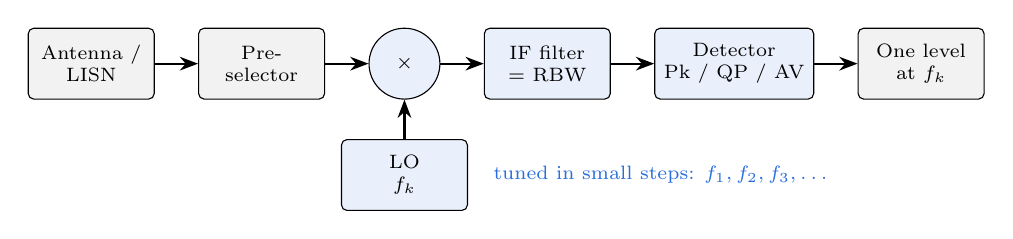
\begin{tikzpicture}[node distance=0.55cm]
  \node[blk=gray]  (ant) {Antenna /\\LISN};
  \node[blk=gray,  right=of ant] (pre) {Pre-\\selector};
  \node[blk=stepc, right=of pre, circle, minimum width=0.9cm] (mix) {$\times$};
  \node[blk=stepc, right=of mix] (if)  {IF filter\\= RBW};
  \node[blk=stepc, right=of if]  (det) {Detector\\Pk / QP / AV};
  \node[blk=gray,  right=of det] (out) {One level\\at $f_k$};
  \node[blk=stepc, below=0.5cm of mix] (lo) {LO\\$f_k$};
  \draw[sig] (ant) -- (pre);
  \draw[sig] (pre) -- (mix);
  \draw[sig] (mix) -- (if);
  \draw[sig] (if)  -- (det);
  \draw[sig] (det) -- (out);
  \draw[sig] (lo)  -- (mix);
  \node[right=0.2cm of lo, font=\scriptsize, align=left, stepc]
    {tuned in small steps: $f_1, f_2, f_3, \dots$};
\end{tikzpicture}

\vspace{2mm}
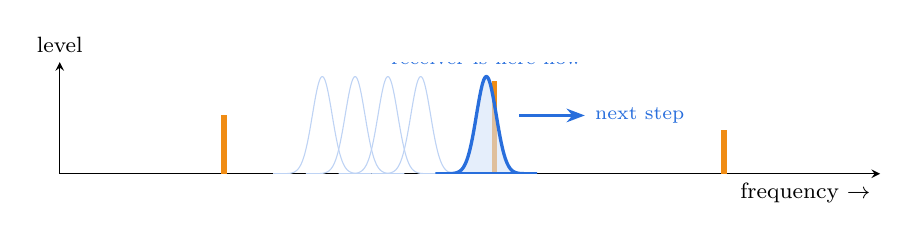
\begin{tikzpicture}
  \begin{axis}[specax, height=3.0cm]
    % emissions
    \addplot[sigc, line width=2pt] coordinates {(2,0) (2,0.6)};
    \addplot[sigc, line width=2pt] coordinates {(5.3,0) (5.3,0.95)};
    \addplot[sigc, line width=2pt] coordinates {(8.1,0) (8.1,0.45)};
    % past steps (faded), current filter (bold)
    \foreach \c in {3.2,3.6,...,4.8} {
      \edef\tmp{\noexpand\addplot[stepc!30, domain=\c-0.6:\c+0.6]
                {\gauss{\c}{0.4}};}
      \tmp
    }
    \addplot[stepc, very thick, fill=stepc!20, fill opacity=0.6,
             domain=4.6:5.8] {\gauss{5.2}{0.4}} \closedcycle;
    \node[stepc, font=\scriptsize, anchor=south] at (axis cs:5.2,1.02)
      {receiver is here now};
    \draw[-{Stealth}, stepc, thick] (axis cs:5.6,0.6) -- (axis cs:6.4,0.6)
      node[right, font=\scriptsize] {next step};
  \end{axis}
\end{tikzpicture}

\small
At each step: tune LO $\rightarrow$ wait for the filter to \textbf{settle}
($\approx$ a few $/\mathrm{RBW}$) $\rightarrow$ \textbf{dwell} with the detector
$\rightarrow$ store one value $\rightarrow$ next step.
\end{frame}

% ======================================================================
\begin{frame}{Stepped scan: how small must the steps be?}

\begin{columns}[c]
\begin{column}{0.52\textwidth}
\begin{tikzpicture}
  \begin{axis}[
      width=7.2cm, height=4.6cm, axis lines=left,
      xmin=-1.3, xmax=1.3, ymin=-13, ymax=1,
      xlabel={offset from filter centre / RBW},
      ylabel={response [dB]},
      label style={font=\footnotesize}, tick label style={font=\scriptsize},
      xtick={-1,-0.5,-0.25,0,0.25,0.5,1},
      xticklabels={$-1$,$-\tfrac12$,,0,$\tfrac14$,$\tfrac12$,1},
      ytick={-12,-6,-1.5,0}, grid=major, grid style={black!15},
      samples=200, domain=-1.3:1.3,
    ]
    \addplot[stepc, very thick] {-6.02*(2*x)^2};
    \addplot[only marks, mark=*, fftc] coordinates {(0.25,-1.505) (0.5,-6.02)};
    \draw[fftc, densely dotted] (axis cs:0.25,-1.505) -- (axis cs:-1.3,-1.505);
    \draw[fftc, densely dotted] (axis cs:0.5,-6.02) -- (axis cs:-1.3,-6.02);
    \node[font=\scriptsize, fftc, anchor=west, fill=white, inner sep=1pt]
      at (axis cs:-1.25,-3.2) {step = RBW/2 $\Rightarrow -1.5$\,dB};
    \node[font=\scriptsize, fftc, anchor=west, fill=white, inner sep=1pt]
      at (axis cs:-1.25,-8.0) {step = RBW $\Rightarrow -6$\,dB};
  \end{axis}
\end{tikzpicture}
\end{column}
\begin{column}{0.46\textwidth}
  A Gaussian filter attenuates a signal that is $\Delta f$ off-centre by
  \[
    A(\Delta f) \approx 6\,\mathrm{dB}\cdot\left(\frac{2\,\Delta f}{\mathrm{RBW}}\right)^{2}
  \]
  The worst case is a signal exactly \alert{between two steps},
  $\Delta f = \text{step}/2$:

  \medskip
  \begin{tabular}{@{}ll@{}}
    \toprule
    Step & Worst-case error \\
    \midrule
    RBW   & $-6$\,dB \\
    RBW/2 & $-1.5$\,dB \\
    RBW/4 & $-0.4$\,dB \\
    \bottomrule
  \end{tabular}

  \medskip
  $\Rightarrow$ in practice: \textbf{step $\le$ RBW/2}, often RBW/3.
\end{column}
\end{columns}

\end{frame}

% ======================================================================
\begin{frame}{Stepped scan: worked example (30\,MHz -- 1\,GHz)}

\begin{columns}[T]
\begin{column}{0.5\textwidth}
  \textbf{Settings} (CISPR band C/D)
  \begin{itemize}
    \item RBW = 120\,kHz, step = 40\,kHz
    \item Number of frequencies:
      \[
        N_f = \frac{1000 - 30\,\mathrm{MHz}}{40\,\mathrm{kHz}} \approx 24\,250
      \]
  \end{itemize}

  \textbf{Scan time} $\approx N_f \times (t_\text{settle} + t_\text{dwell})$
\end{column}
\begin{column}{0.47\textwidth}
  \centering
  \begin{tabular}{@{}lrr@{}}
    \toprule
    Detector & dwell & scan time \\
    \midrule
    Peak       & 1\,ms   & $\approx 25$\,s \\
    Average    & 100\,ms & $\approx 40$\,min \\
    Quasi-peak & 1\,s    & \alert{$\approx 6.7$\,h} \\
    \bottomrule
  \end{tabular}

  \medskip
  \scriptsize (plus settling / overhead per step,\\and $\times 2$ for two
  antenna polarisations, $\times$ turntable angles, $\times$ antenna heights \dots)
\end{column}
\end{columns}

\bigskip
\begin{alertblock}{Two consequences}
  \begin{enumerate}
    \item A full QP scan is practically impossible $\Rightarrow$ one does a quick
          Peak pre-scan and measures QP only at a few suspect frequencies.
    \item At any instant the receiver looks at only $120\,\mathrm{kHz}$ of
          $970\,\mathrm{MHz}$ $\approx$ \alert{0.01\,\%} of the band.
          Short or intermittent emissions are easily \textbf{missed}.
  \end{enumerate}
\end{alertblock}

\end{frame}

% ======================================================================
\begin{frame}{Time-domain scan: sample first, compute the spectrum later}

\centering
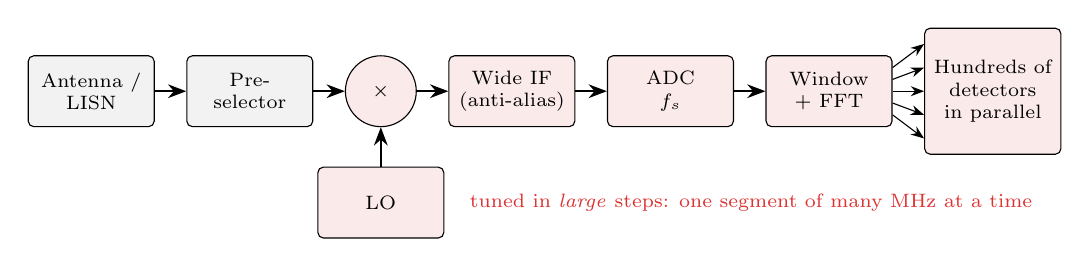
\begin{tikzpicture}[node distance=0.4cm]
  \node[blk=gray]  (ant) {Antenna /\\LISN};
  \node[blk=gray,  right=of ant] (pre) {Pre-\\selector};
  \node[blk=fftc, right=of pre, circle, minimum width=0.9cm] (mix) {$\times$};
  \node[blk=fftc, right=of mix] (if)  {Wide IF\\(anti-alias)};
  \node[blk=fftc, right=of if]  (adc) {ADC\\$f_s$};
  \node[blk=fftc, right=of adc] (fft) {Window\\+ FFT};
  \node[blk=fftc, right=of fft, minimum height=1.6cm] (det)
    {Hundreds of\\detectors\\in parallel};
  \node[blk=fftc, below=0.5cm of mix] (lo) {LO};
  \draw[sig] (ant) -- (pre);
  \draw[sig] (pre) -- (mix);
  \draw[sig] (mix) -- (if);
  \draw[sig] (if)  -- (adc);
  \draw[sig] (adc) -- (fft);
  \foreach \dy in {-0.6,-0.3,0,0.3,0.6}
    \draw[-{Stealth}] ($(fft.east)+(0,\dy*0.5)$) -- ($(det.west)+(0,\dy)$);
  \draw[sig] (lo)  -- (mix);
  \node[right=0.2cm of lo, font=\scriptsize, align=left, fftc]
    {tuned in \emph{large} steps: one segment of many MHz at a time};
\end{tikzpicture}

\vspace{2mm}
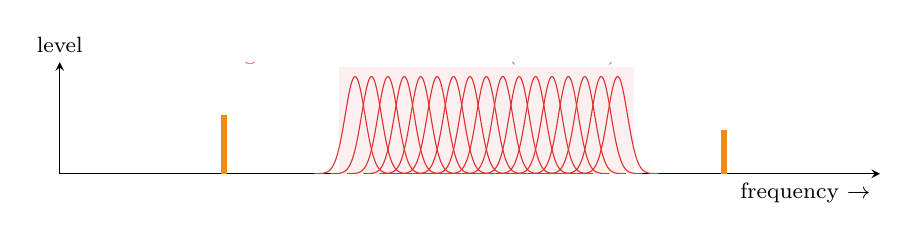
\begin{tikzpicture}
  \begin{axis}[specax, height=3.0cm]
    \addplot[sigc, line width=2pt] coordinates {(2,0) (2,0.6)};
    \addplot[sigc, line width=2pt] coordinates {(5.3,0) (5.3,0.95)};
    \addplot[sigc, line width=2pt] coordinates {(8.1,0) (8.1,0.45)};
    \fill[fftc!8] (axis cs:3.4,0) rectangle (axis cs:7.0,1.1);
    \foreach \c in {3.6,3.8,...,6.8} {
      \edef\tmp{\noexpand\addplot[fftc, thin, domain=\c-0.5:\c+0.5]
                {\gauss{\c}{0.4}};}
      \tmp
    }
    \node[fftc, font=\scriptsize, anchor=south] at (axis cs:5.2,1.02)
      {one segment = all these ``filters'' (FFT bins) at the same time};
  \end{axis}
\end{tikzpicture}

\small
The FFT acts like a \alert{bank of RBW filters} working simultaneously.
Detectors (Pk, QP, AV) are then applied to every bin in software/FPGA.
\end{frame}

% ======================================================================
\begin{frame}{Time-domain scan: getting the right RBW out of an FFT}

\begin{columns}[T]
\begin{column}{0.52\textwidth}
  \small
  An FFT of $N$ samples taken at rate $f_s$ covers a record of length
  \[ T = N/f_s \]
  and gives bins spaced $\Delta f_\text{bin} = 1/T$.

  \medskip
  The \textbf{window} (Gaussian / Hann-like) turns each bin into a filter
  with 6\,dB bandwidth
  \[ \mathrm{RBW} \approx k\cdot\frac{f_s}{N} = \frac{k}{T},
     \qquad k\approx 2 \text{ (Hann)} \]

  \vspace{-2mm}
  \begin{block}{Key insight}
    \small A filter of bandwidth $B$ needs a time $\sim 1/B$ to ``see'' a
    signal -- \emph{the same physics} as the settling time in the
    stepped receiver.
  \end{block}
\end{column}
\begin{column}{0.45\textwidth}
  \textbf{Example} (band C/D, RBW 120\,kHz)

  \smallskip
  \footnotesize
  \begin{tabular}{@{}ll@{}}
    \toprule
    I/Q sample rate  & $f_s = 32$\,MS/s \\
    FFT length       & $N = 512$ \\
    Record length    & $T = 16\,\mu$s \\
    Bin spacing      & $1/T = 62.5$\,kHz $\approx$ RBW/2 \\
    RBW (Hann)       & $2/T = 125$\,kHz $\approx 120$\,kHz \\
    Usable span      & $\approx 25$\,MHz (80\,\% of $f_s$) \\
    Bins per segment & $\approx 400$ \\
    \bottomrule
  \end{tabular}

  \medskip
  \small
  $\Rightarrow$ 400 frequencies measured in the time a stepped receiver
  measures \alert{one}.
\end{column}
\end{columns}

\end{frame}

% ======================================================================
\begin{frame}{Time-domain scan: overlapping FFTs -- no gaps in time}

\begin{columns}[c]
\begin{column}{0.55\textwidth}
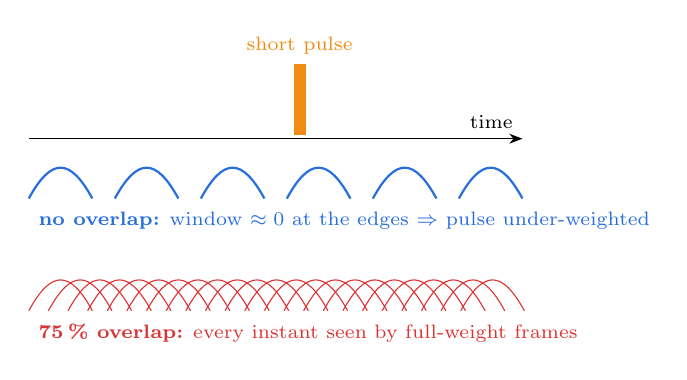
\begin{tikzpicture}[x=1cm, y=1cm, scale=0.95]
  % time axis
  \draw[-{Stealth}] (0,0) -- (6.6,0) node[above left, font=\scriptsize] {time};
  % a short pulse
  \fill[sigc] (3.55,0.05) rectangle (3.7,1.0);
  \node[sigc, font=\scriptsize, above] at (3.62,1.0) {short pulse};

  % non-overlapping frames
  \foreach \i in {0,...,5} {
    \draw[stepc, thick] (\i*1.15,-0.8) .. controls (\i*1.15+0.3,-0.25)
      and (\i*1.15+0.55,-0.25) .. (\i*1.15+0.85,-0.8);
  }
  \node[stepc, font=\scriptsize, anchor=west] at (0,-1.1)
    {\textbf{no overlap:} window $\approx 0$ at the edges $\Rightarrow$ pulse under-weighted};

  % overlapping frames
  \foreach \i in {0,...,22} {
    \pgfmathsetmacro\s{\i*0.2625}
    \draw[fftc, thin] (\s,-2.3) .. controls (\s+0.3,-1.75)
      and (\s+0.55,-1.75) .. (\s+0.85,-2.3);
  }
  \node[fftc, font=\scriptsize, anchor=west] at (0,-2.6)
    {\textbf{75\,\% overlap:} every instant seen by full-weight frames};
\end{tikzpicture}
\end{column}
\begin{column}{0.42\textwidth}
  \small
  \begin{itemize}
    \item The window tapers the record ends, so consecutive FFTs must
          \textbf{overlap} to observe the signal \emph{gaplessly}.
    \item This is required for correct \textbf{QP / pulse} weighting
          (CISPR pulse-response tests).
    \item Cost: lots of computation.
  \end{itemize}

  \medskip
  \footnotesize
  Example: $N=512$, $f_s = 32$\,MS/s, 90\,\% overlap
  \[ \frac{f_s}{N(1-0.9)} \approx 625\,000 \text{ FFTs/s} \]
  $\Rightarrow$ done in an \alert{FPGA}, not a PC.
\end{column}
\end{columns}

\end{frame}

% ======================================================================
\begin{frame}{Same example with a time-domain scan (30\,MHz -- 1\,GHz)}

\begin{columns}[T]
\begin{column}{0.48\textwidth}
  \begin{itemize}
    \item Segment width $\approx 25$\,MHz
    \item Number of segments:
      \[ \frac{970\,\mathrm{MHz}}{25\,\mathrm{MHz}} \approx 39 \]
    \item Every segment gets the \emph{full} dwell time -- for all its
          $\approx 400$ bins at once.
  \end{itemize}
  \scriptsize
  (Modern receivers offer segment widths of hundreds of MHz, making it
  even faster.)
\end{column}
\begin{column}{0.49\textwidth}
  \centering
  \begin{tabular}{@{}lrrr@{}}
    \toprule
    Detector & dwell & \textcolor{stepc}{stepped} & \textcolor{fftc}{FFT} \\
    \midrule
    Peak       & 1\,ms   & 25\,s      & $<1$\,s \\
    Average    & 100\,ms & 40\,min    & 4\,s \\
    Quasi-peak & 1\,s    & 6.7\,h     & \alert{40\,s} \\
    \bottomrule
  \end{tabular}

  \medskip
  \small Speed-up $\approx$ number of bins per segment
  ($\sim 10^2$--$10^4$).
\end{column}
\end{columns}

\bigskip
\begin{exampleblock}{What this changes in practice}
  A \textbf{full quasi-peak scan} of the whole band becomes feasible, and with
  the time saved one can afford \emph{longer} dwell times -- which is exactly
  what catches intermittent emissions.
\end{exampleblock}

\end{frame}

% ======================================================================
\begin{frame}{Example: catching an intermittent emission}

Emission at $f_0$: a \textbf{10\,ms burst once per second} (e.g.\ a relay,
a motor controller, a data packet).

\medskip
\centering
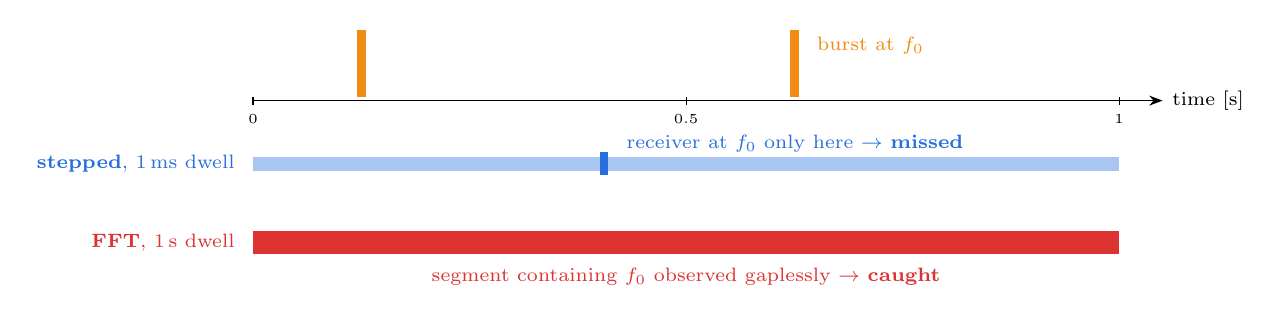
\begin{tikzpicture}[x=11cm, y=1cm]
  \draw[-{Stealth}] (0,0) -- (1.05,0) node[right, font=\scriptsize] {time [s]};
  \foreach \t in {0,0.5,1} \draw (\t,0.05) -- (\t,-0.05)
    node[below, font=\tiny] {\t};
  % bursts
  \foreach \t in {0.12, 0.62} \fill[sigc] (\t,0.05) rectangle (\t+0.01,0.9);
  \node[sigc, font=\scriptsize, anchor=west] at (0.64,0.7) {burst at $f_0$};

  % stepped
  \node[stepc, font=\scriptsize, anchor=east] at (-0.01,-0.8)
    {\textbf{stepped}, 1\,ms dwell};
  \draw[stepc!40, line width=5pt] (0,-0.8) -- (1,-0.8);
  \fill[stepc] (0.40,-0.95) rectangle (0.41,-0.65);
  \node[stepc, font=\scriptsize, anchor=west] at (0.42,-0.55)
    {receiver at $f_0$ only here $\rightarrow$ \textbf{missed}};

  % fft
  \node[fftc, font=\scriptsize, anchor=east] at (-0.01,-1.8)
    {\textbf{FFT}, 1\,s dwell};
  \fill[fftc] (0,-1.95) rectangle (1,-1.65);
  \node[fftc, font=\scriptsize, anchor=north] at (0.5,-2.0)
    {segment containing $f_0$ observed gaplessly $\rightarrow$ \textbf{caught}};
\end{tikzpicture}

\raggedright
\medskip
\small
Probability that the stepped receiver sees the burst at all:
\[
  P \approx \frac{t_\text{burst} + t_\text{dwell}}{T_\text{repeat}}
    = \frac{10\,\mathrm{ms} + 1\,\mathrm{ms}}{1\,\mathrm{s}} \approx
    \alert{1\,\%}
  \quad\text{vs.}\quad P_\text{FFT} = 100\,\%
\]
\end{frame}

% ======================================================================
\begin{frame}{Stepped scan: advantages and drawbacks}

\begin{columns}[T]
\begin{column}{0.49\textwidth}
  \textcolor{okc}{\large\textbf{Advantages}}
  \small
  \begin{itemize}
    \item[\plus] The \textbf{reference method}: a direct implementation of the
                 CISPR~16-1-1 receiver model -- easy to understand and verify
    \item[\plus] \textbf{High dynamic range}: only one narrow band reaches the
                 detector; a strong signal elsewhere does not load the ADC
    \item[\plus] Robust with \textbf{broadband impulsive} signals
                 (little overload risk)
    \item[\plus] Any detector / dwell / step per frequency, simple hardware
    \item[\plus] Universally accepted by all standards and labs
  \end{itemize}
\end{column}
\begin{column}{0.49\textwidth}
  \textcolor{badc}{\large\textbf{Drawbacks}}
  \small
  \begin{itemize}
    \item[\minus] \textbf{Slow}: time $\propto$ number of frequencies
                  $\times$ dwell (QP: hours)
    \item[\minus] Sees only $\approx 0.01\,\%$ of the band at a time
                  $\Rightarrow$ \textbf{misses intermittent} and drifting
                  emissions
    \item[\minus] Temptation to use coarse steps / short dwell to save time
                  $\Rightarrow$ under-reads levels
    \item[\minus] Long tests: EUT must run stable for hours, occupies
                  the chamber
  \end{itemize}
\end{column}
\end{columns}

\end{frame}

% ======================================================================
\begin{frame}{Time-domain (FFT) scan: advantages and drawbacks}

\begin{columns}[T]
\begin{column}{0.49\textwidth}
  \textcolor{okc}{\large\textbf{Advantages}}
  \small
  \begin{itemize}
    \item[\plus] \textbf{Very fast}: 100--10\,000$\times$; full-band
                 QP / CISPR-AV scans in seconds--minutes
    \item[\plus] \textbf{Gapless} observation: catches intermittent,
                 hopping and transient emissions
    \item[\plus] Fine frequency grid for free (many bins)
    \item[\plus] Enables real-time spectrum and spectrogram views --
                 great for \textbf{debugging}
    \item[\plus] Accepted for compliance by CISPR~16-1-1 if the receiver
                 meets the same requirements (pulse response, accuracy)
  \end{itemize}
\end{column}
\begin{column}{0.49\textwidth}
  \textcolor{badc}{\large\textbf{Drawbacks}}
  \small
  \begin{itemize}
    \item[\minus] Whole segment shares one ADC $\Rightarrow$ a \textbf{strong
                  signal} or broadband pulse can \textbf{overload} or reduce
                  dynamic range; needs good preselection
    \item[\minus] Low-repetition \textbf{impulsive} signals are demanding:
                  window, overlap and ADC headroom must be right
    \item[\minus] Heavy DSP (FPGA) $\Rightarrow$ expensive, more complex to verify
    \item[\minus] Possible artefacts: ADC spurs, leakage, segment edges
    \item[\minus] Check that the product standard / accreditation accepts it
  \end{itemize}
\end{column}
\end{columns}

\end{frame}

% ======================================================================
\begin{frame}{Summary and typical workflow}

\centering
\footnotesize
\begin{tabular}{@{}lll@{}}
  \toprule
  & \textcolor{stepc}{\textbf{Stepped scan}}
  & \textcolor{fftc}{\textbf{Time-domain (FFT) scan}} \\
  \midrule
  Principle        & one RBW filter, tuned in steps
                   & FFT = parallel RBW filter bank \\
  Observed at once & one frequency ($\approx 0.01\,\%$ of band)
                   & a segment, MHz wide \\
  Full QP scan 30\,MHz--1\,GHz & hours & $<1$ minute \\
  Intermittent signals & easily missed & caught (gapless) \\
  Dynamic range    & best & good, ADC-limited per segment \\
  Complexity       & low  & high (FPGA) \\
  \bottomrule
\end{tabular}

\medskip
\raggedright
\small
\textbf{Typical modern workflow}
\begin{enumerate}
  \item \textcolor{fftc}{FFT pre-scan} with Peak + Average over the whole band
        (seconds), all polarisations / heights / angles
  \item Pick the frequencies close to the limit line
  \item \textbf{Final measurement} with QP and CISPR-AV at those frequencies
        (single-frequency or stepped, maximising EUT position)
  \item Suspect overload? Add 10\,dB attenuation: a real emission reading
        stays the same (after correction), an overload artefact does not
\end{enumerate}

\end{frame}

\end{document}
